\documentclass[14pt, a4paper]{extarticle}
\usepackage{mospolytech_coursework}
\usepackage{xurl}
\usepackage{tocloft}
\sloppy
\setlength{\tabcolsep}{4pt}
\renewcommand{\arraystretch}{1.15}
\renewcommand{\cftsecfont}{\fontsize{12.5}{14}\selectfont}
\renewcommand{\cftsubsecfont}{\fontsize{12.5}{14}\selectfont}
\renewcommand{\cftsecpagefont}{\fontsize{12.5}{14}\selectfont}
\renewcommand{\cftsubsecpagefont}{\fontsize{12.5}{14}\selectfont}
\setlength{\cftbeforesecskip}{0pt}
\lstset{basicstyle=\small\rmfamily,columns=fullflexible,breaklines=true,keepspaces=true}

% Определение данных
\newcommand{\theme}{%
    Разработка веб-приложения для хранения, систематизации и выдачи учебных материалов%
}
\newcommand{\subject}{Разработка веб-приложений}
\newcommand{\student}{Николаев Алексей Владимирович}
\newcommand{\group}{241-3211}
\newcommand{\teacher}{Кружалов Алексей Сергеевич}

\begin{document}

% Титульный лист
\include{title}

% Задание
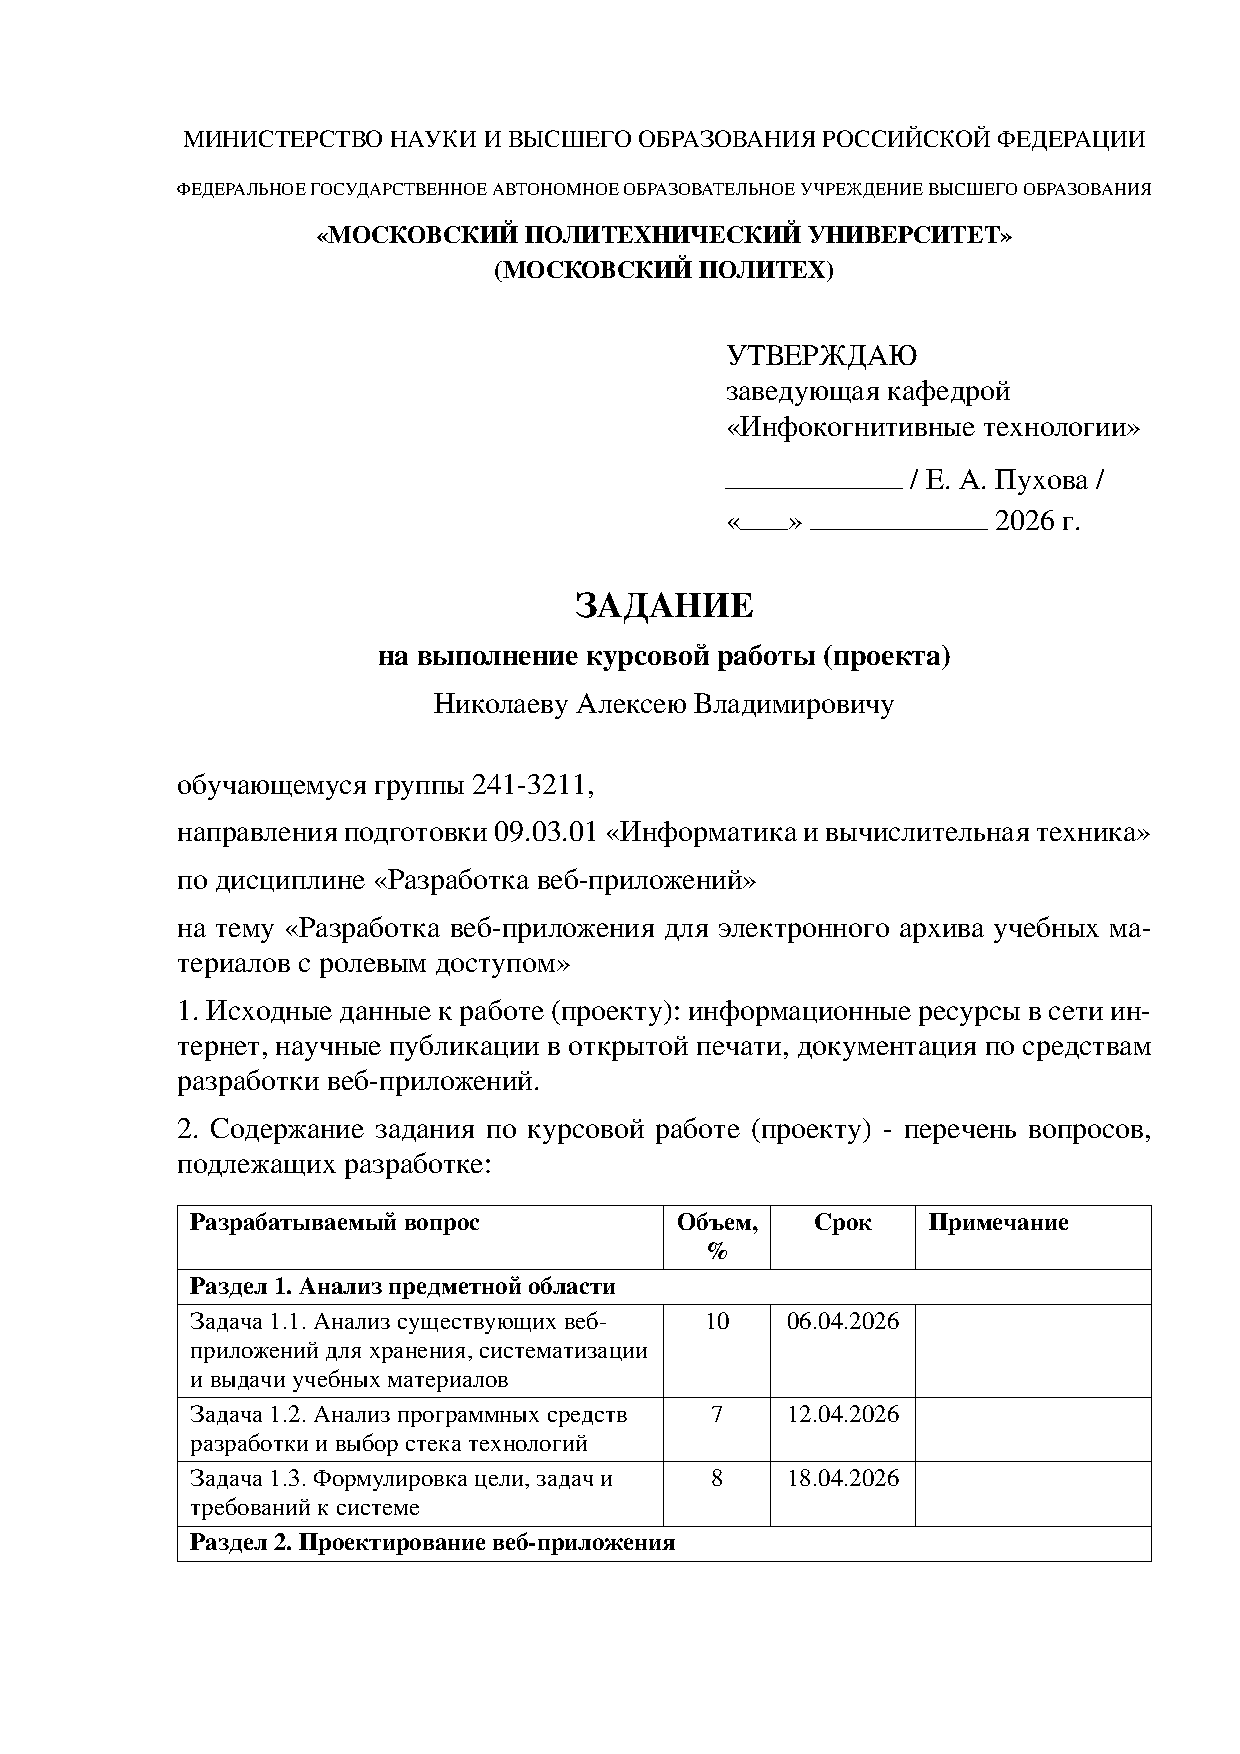
\includepdf[pages=-]{task.pdf}

% Содержание
\tableofcontents

% Введение
\section*{Введение}
\addcontentsline{toc}{section}{Введение}

В условиях активного использования электронных образовательных ресурсов задача хранения, систематизации и предоставления учебных материалов приобретает особую актуальность. В учебном процессе преподаватели и студенты постоянно работают с лекциями, методическими указаниями, лабораторными заданиями, презентациями и иными файлами, которые должны быть доступны в удобной, структурированной и безопасной форме. При отсутствии единого веб-инструмента материалы нередко хранятся разрозненно: в облачных сервисах, мессенджерах, на личных страницах преподавателей или в локальных каталогах. Это затрудняет поиск нужной информации, усложняет контроль актуальности файлов и не позволяет полноценно разграничивать доступ пользователей.

Целью курсового проекта является разработка веб-приложения для хранения, систематизации и выдачи учебных материалов с учетом роли пользователя. Для достижения данной цели в работе были решены задачи анализа предметной области, выбора стека технологий, проектирования структуры приложения и модели данных, а также реализации механизмов аутентификации, авторизации, проверки прав доступа, CRUD-операций, загрузки и скачивания файлов и формирования статистики.

Объектом исследования является процесс электронного хранения и предоставления учебных материалов в рамках образовательной деятельности. Предметом исследования выступают методы и средства проектирования и разработки веб-приложения, обеспечивающего централизованную работу с такими материалами. Практическая значимость проекта заключается в создании работоспособного программного решения, которое может использоваться как основа для учебного архива материалов кафедры, дисциплины или отдельного курса.

% Основная часть
\section*{Глава 1. Анализ предметной области}
\addcontentsline{toc}{section}{Глава 1. Анализ предметной области}
\stepcounter{section}

В данной главе выполняется анализ предметной области, связанной с хранением, систематизацией и публикацией учебных материалов в электронном виде. Рассматриваются существующие подходы и программные средства, формулируются цель, задачи и основные требования к разрабатываемому веб-приложению.

\subsection{Анализ существующих веб-приложений для хранения,\ систематизации и публикации учебных материалов}

В современных образовательных организациях учебные материалы представлены преимущественно в электронном виде. К таким материалам относятся лекции, лабораторные работы, методические указания, практические задания, презентации, шаблоны отчетов и иные вспомогательные документы. Все перечисленные данные должны быть доступны преподавателям и студентам в удобной и структурированной форме, а также поддерживаться в актуальном состоянии в течение учебного процесса.

На практике хранение учебных материалов часто организовано нецентрализованно. Документы размещаются в различных облачных сервисах, мессенджерах, на личных страницах преподавателей или в файловых каталогах. Подобный подход приводит к нескольким типичным проблемам. Во-первых, усложняется поиск нужного материала, так как пользователь вынужден обращаться к нескольким источникам. Во-вторых, отсутствует единая структура хранения, что затрудняет систематизацию материалов по дисциплинам, темам, видам занятий или авторам. В-третьих, при отсутствии ролевого разграничения доступа возрастает риск несанкционированного изменения или удаления данных. Наконец, становится затруднительным контроль актуальности материалов и учет действий пользователей.

Существующие программные решения частично закрывают обозначенные потребности. К наиболее распространенным подходам относятся облачные файловые хранилища, системы дистанционного обучения и внутренние корпоративные порталы кафедр и учебных подразделений.

\begin{center}
\begin{tabularx}{0.96\textwidth}{>{\raggedright\arraybackslash}p{3.8cm} >{\raggedright\arraybackslash}X >{\raggedright\arraybackslash}X}
\toprule
\textbf{Тип решения} & \textbf{Преимущества} & \textbf{Недостатки} \\
\midrule
Облачные файловые хранилища & Простая загрузка и скачивание файлов, совместный доступ, привычный интерфейс & Слабая предметно-ориентированная структура, ограниченные возможности ролевого разграничения и статистики \\
Системы дистанционного обучения & Поддержка учебного процесса, разграничение доступа, публикация материалов и заданий & Избыточность функциональности для узкой задачи электронного архива, более сложное сопровождение \\
Внутренние сайты и порталы кафедр & Возможность адаптации под локальные потребности, относительная простота публикации & Отсутствие единого подхода к моделированию данных, слабая поддержка CRUD-операций и аналитики \\
\bottomrule
\end{tabularx}
\end{center}

Облачные сервисы, такие как Google Drive и аналогичные решения, удобны для обмена файлами, однако ориентированы прежде всего на файловое хранение. В них отсутствует выраженная модель предметной области, которая необходима для учебного архива: категории материалов, авторство, ролевой доступ, фильтрация и агрегирование данных.

Системы дистанционного обучения, например Moodle и аналогичные платформы, предоставляют широкие возможности для организации учебного процесса. Они позволяют публиковать учебные материалы, управлять доступом и вести учет активности. Однако подобные решения во многих случаях являются слишком сложными для задач компактного архива учебных материалов. Для учебного проекта их архитектура и функциональная насыщенность могут быть избыточными.

Внутренние сайты кафедр и учебных подразделений обычно создаются под локальные задачи. Такие решения могут быть удобны в использовании, но часто развиваются бессистемно. В результате возникают трудности при расширении структуры данных, организации прав доступа и поддержке целостности информации.

Таким образом, проведенный анализ показывает целесообразность разработки отдельного веб-приложения, ориентированного именно на хранение, систематизацию и публикацию учебных материалов. Такое приложение должно быть проще полнофункциональных образовательных платформ, но при этом содержать обязательные механизмы аутентификации, авторизации, ролевого разграничения доступа, CRUD-операций, загрузки и скачивания файлов, а также базовой статистической обработки данных.

\subsection{Анализ программных средств разработки и выбор стека технологий}

Для реализации веб-приложения необходимо выбрать программные средства, позволяющие создать серверную логику, пользовательский интерфейс, механизм аутентификации, доступ к базе данных и обработку файлов. Поскольку проект выполняется в учебных целях, основными критериями выбора являются простота освоения, доступность документации, достаточность функциональности и удобство поэтапной разработки.

В качестве языка программирования выбран Python. Данный язык обладает простым и читаемым синтаксисом, широко используется при разработке веб-приложений и имеет большой набор библиотек для решения прикладных задач. В качестве альтернативы можно рассматривать Rust, который обеспечивает высокую производительность и безопасность памяти, однако его использование требует более глубокого понимания низкоуровневых механизмов и усложняет разработку учебного проекта. Поэтому для данной работы выбран Python, так как он позволяет быстрее реализовать основную логику приложения и сосредоточиться на предметной области.

В качестве веб-фреймворка выбран Flask. Он представляет собой легковесное средство разработки веб-приложений, позволяющее реализовать маршрутизацию, шаблонизацию страниц, обработку форм, работу с файлами и интеграцию со сторонними библиотеками. В качестве альтернативы можно использовать Django, который предоставляет больше встроенных возможностей, включая административную панель, ORM и готовую структуру проекта. Однако для небольшого учебного приложения Django может быть избыточным и требовать большего объема настройки. Flask выбран потому, что он проще по структуре и удобен для поэтапной реализации необходимых функций.

Для аутентификации пользователей и управления сессиями выбран модуль Flask-Login. Он предоставляет готовые механизмы входа в систему, выхода из нее, восстановления текущего пользователя и ограничения доступа к маршрутам для неавторизованных пользователей. В качестве альтернативы можно было реализовать механизм аутентификации самостоятельно с использованием сессий Flask. Однако самостоятельная реализация потребовала бы больше кода и увеличила бы вероятность ошибок при проверке авторизации. Flask-Login выбран потому, что он упрощает реализацию входа пользователей и делает работу с текущим пользователем более удобной и надежной.

Для работы с базой данных используется Flask-SQLAlchemy. Библиотека обеспечивает объектно-реляционное отображение, позволяя описывать сущности в виде Python-классов и выполнять операции с данными на уровне моделей. В качестве альтернативы можно использовать прямые SQL-запросы через модуль sqlite3. Такой подход дает больше контроля над запросами, однако усложняет поддержку кода и требует вручную описывать многие операции с данными. Flask-SQLAlchemy выбран потому, что он упрощает реализацию CRUD-интерфейса, уменьшает количество повторяющегося кода и делает структуру приложения более понятной.

В качестве системы управления базой данных выбрана SQLite. Ее преимуществами являются простота настройки, отсутствие необходимости устанавливать отдельный сервер базы данных и достаточность возможностей для учебного проекта. В качестве альтернативы можно использовать PostgreSQL, который лучше подходит для крупных и нагруженных приложений, поддерживает расширенные возможности и многопользовательскую работу. Однако для учебного проекта использование PostgreSQL усложнило бы настройку и развертывание. SQLite выбрана потому, что она не требует отдельного сервера и позволяет быстро приступить к разработке приложения.

Для построения пользовательского интерфейса используются HTML, CSS, Jinja2 и Bootstrap. HTML и CSS применяются для описания структуры и внешнего вида страниц, Jinja2 позволяет формировать динамические страницы на стороне сервера, а Bootstrap обеспечивает единый и аккуратный внешний вид интерфейса. В качестве альтернативы можно использовать отдельный JavaScript-фреймворк, например React. Такой подход удобен для сложных интерактивных интерфейсов, однако требует разработки отдельной клиентской части и дополнительной настройки взаимодействия с сервером. Для данного проекта выбран серверный рендеринг с Jinja2 и Bootstrap, так как он проще в реализации и полностью соответствует требованиям учебного веб-приложения.

\begin{center}
\footnotesize\begin{tabularx}{0.96\textwidth}{>{\raggedright\arraybackslash}p{4.1cm} >{\raggedright\arraybackslash}p{3.1cm} >{\raggedright\arraybackslash}X}
\toprule
\textbf{Компонент} & \textbf{Выбранное средство} & \textbf{Причина выбора} \\
\midrule
Язык программирования & Python & Простота синтаксиса, высокая скорость разработки, хорошая документация \\
Веб-фреймворк & Flask & Легковесность, гибкость, удобство для учебного проекта \\
Аутентификация & Flask-Login & Готовые механизмы входа, выхода и работы с пользовательской сессией \\
Доступ к БД & Flask-SQLAlchemy & Удобная работа с моделями, ORM-подход, упрощение CRUD-операций \\
СУБД & SQLite & Простая настройка, отсутствие отдельного серверного ПО, достаточность для проекта \\
Шаблоны и интерфейс & Jinja2, Bootstrap & Динамическая генерация страниц и единый визуальный стиль \\
Работа с файлами & Средства Flask и Werkzeug & Простая загрузка, сохранение и скачивание файлов \\
\bottomrule
\end{tabularx}
\end{center}

Таким образом, выбранный стек технологий включает Python, Flask, Flask-Login, Flask-SQLAlchemy, SQLite, Jinja2 и Bootstrap.

\subsection{Формулировка цели, задач и требований к системе}

Целью курсового проекта является разработка веб-приложения для хранения, систематизации и публикации учебных материалов с разграничением прав доступа пользователей в зависимости от их роли.

Для достижения поставленной цели необходимо решить следующие задачи:

\begin{itemize}[leftmargin=1.25cm]
    \item проанализировать предметную область хранения и предоставления учебных материалов;
    \item определить категории пользователей системы и их права доступа;
    \item выделить основные сущности предметной области и связи между ними;
    \item спроектировать структуру базы данных и интерфейс веб-приложения;
    \item реализовать аутентификацию и авторизацию пользователей;
    \item реализовать систему проверки прав доступа в соответствии с ролью пользователя;
    \item реализовать CRUD-интерфейс для пользователей, категорий и материалов;
    \item реализовать загрузку, скачивание и удаление файлов учебных материалов;
    \item реализовать агрегирование данных и формирование статистики;
    \item выполнить тестирование и подготовить пояснительную документацию.
\end{itemize}

В рамках системы выделяются следующие категории пользователей:

\begin{center}
\small\begin{tabularx}{0.96\textwidth}{>{\raggedright\arraybackslash}p{4.2cm} >{\raggedright\arraybackslash}X}
\toprule
\textbf{Роль} & \textbf{Основные функции} \\
\midrule
Администратор & Управление пользователями, категориями и всеми материалами, просмотр статистики, полный контроль над системой \\
Преподаватель & Создание и редактирование собственных материалов, загрузка и удаление файлов, просмотр категорий и материалов \\
Студент & Просмотр списка материалов, открытие карточек материалов, скачивание прикрепленных файлов \\
\bottomrule
\end{tabularx}
\end{center}

В приложении представлены следующие сущности:

\begin{center}
\begin{tabularx}{0.96\textwidth}{>{\raggedright\arraybackslash}p{3.4cm} >{\raggedright\arraybackslash}X}
\toprule
\textbf{Сущность} & \textbf{Назначение} \\
\midrule
Пользователь & Хранение сведений об учетной записи, логине, пароле, ФИО и роли \\
Роль & Определение уровня прав доступа пользователя \\
Категория & Классификация учебных материалов по тематике или типу \\
Материал & Основная сущность архива, содержащая название, описание, автора и категорию \\
Файл & Сведения о прикрепленном файле учебного материала и его хранении \\
\bottomrule
\end{tabularx}
\end{center}

К основным функциональным требованиям относятся:

\begin{itemize}[leftmargin=1.25cm]
    \item регистрация и аутентификация пользователей администраторами системы;
    \item авторизация и разграничение прав доступа по ролям;
    \item создание, просмотр, редактирование и удаление пользователей;
    \item создание, просмотр, редактирование и удаление категорий;
    \item создание, просмотр, редактирование и удаление материалов;
    \item загрузка, скачивание и удаление файлов, связанных с материалами;
    \item фильтрация и поиск материалов;
    \item формирование агрегированных данных и статистики.
\end{itemize}

К основным нефункциональным требованиям относятся удобство интерфейса, корректная работа в современных браузерах, поддержание целостности данных, ограничение доступа в соответствии с ролями и возможность дальнейшего расширения системы.
\section*{Глава 2. Проектирование веб-приложения}
\addcontentsline{toc}{section}{Глава 2. Проектирование веб-приложения}
\stepcounter{section}

На данном этапе определяются роли пользователей и их права доступа, проектируются основные сценарии использования системы, формируется модель данных и описывается структура интерфейса. Результаты проектирования служат основой для последующей программной реализации системы.

\subsection{Определение ролей пользователей и прав доступа}

Для обеспечения безопасной и логичной работы системы необходимо заранее определить категории пользователей и круг доступных им действий. В проектируемом приложении используются три роли: администратор, преподаватель и студент.

Администратор обладает максимальным набором прав и отвечает за общее сопровождение системы. Он управляет учетными записями пользователей, ролями, категориями и всеми материалами, а также имеет доступ к просмотру статистики. Преподаватель работает с учебными материалами: создает их, редактирует собственные записи, прикрепляет файлы и при необходимости удаляет их. Студент использует приложение только как средство получения учебной информации, поэтому для него доступен просмотр материалов и скачивание файлов.

Матрица прав доступа представлена в таблице.

\begin{center}
\small\begin{tabularx}{0.96\textwidth}{>{\raggedright\arraybackslash}p{7.8cm} >{\centering\arraybackslash}p{1.6cm} >{\centering\arraybackslash}p{2.1cm} >{\centering\arraybackslash}p{2.0cm}}
\toprule
\textbf{Функция} & \textbf{Адм.} & \textbf{Препод.} & \textbf{Студ.} \\
\midrule
Вход в систему и выход из нее & + & + & + \\
Просмотр списка материалов & + & + & + \\
Просмотр карточки материала & + & + & + \\
Создание материалов & + & + & -- \\
Редактирование собственных материалов & + & + & -- \\
Удаление материалов & + & + & -- \\
Загрузка файлов к материалам & + & + & -- \\
Удаление файлов из материалов & + & + & -- \\
Просмотр категорий & + & + & -- \\
Управление категориями & + & -- & -- \\
Управление пользователями & + & -- & -- \\
Просмотр статистики & + & -- & -- \\
\bottomrule
\end{tabularx}
\end{center}

Выбранное распределение прав позволяет сохранить необходимый уровень безопасности и при этом не усложняет взаимодействие пользователей с системой.

\subsection{Проектирование функциональности приложения и сценариев использования}

Проектируемое приложение должно обеспечивать базовый набор пользовательских сценариев, связанных с управлением учебными материалами. На этапе проектирования были выделены основные функции системы: вход пользователя в систему, управление учетными записями, управление категориями, работа с материалами и файлами, а также просмотр статистики.

Основные пользовательские сценарии можно описать следующим образом:

\begin{itemize}[leftmargin=1.25cm]
    \item администратор входит в систему, создает пользователей, назначает им роли, управляет категориями и контролирует наполнение архива;
    \item преподаватель входит в систему, создает новый материал, заполняет его описание, выбирает категорию и прикрепляет файлы;
    \item преподаватель при необходимости редактирует собственный материал, обновляет информацию и удаляет ненужные файлы;
    \item студент входит в систему, просматривает список материалов, открывает карточку нужного материала и скачивает прикрепленный файл;
    \item администратор открывает страницу статистики и анализирует распределение материалов по категориям, авторам и ролям пользователей.
\end{itemize}

Для наглядного представления взаимодействия пользователей с системой в проект была включена диаграмма вариантов использования. На диаграмме отражены основные акторы системы --- администратор, преподаватель и студент --- и показаны ключевые действия, которые доступны каждой роли.

\begin{figure}[h!]
    \centering
    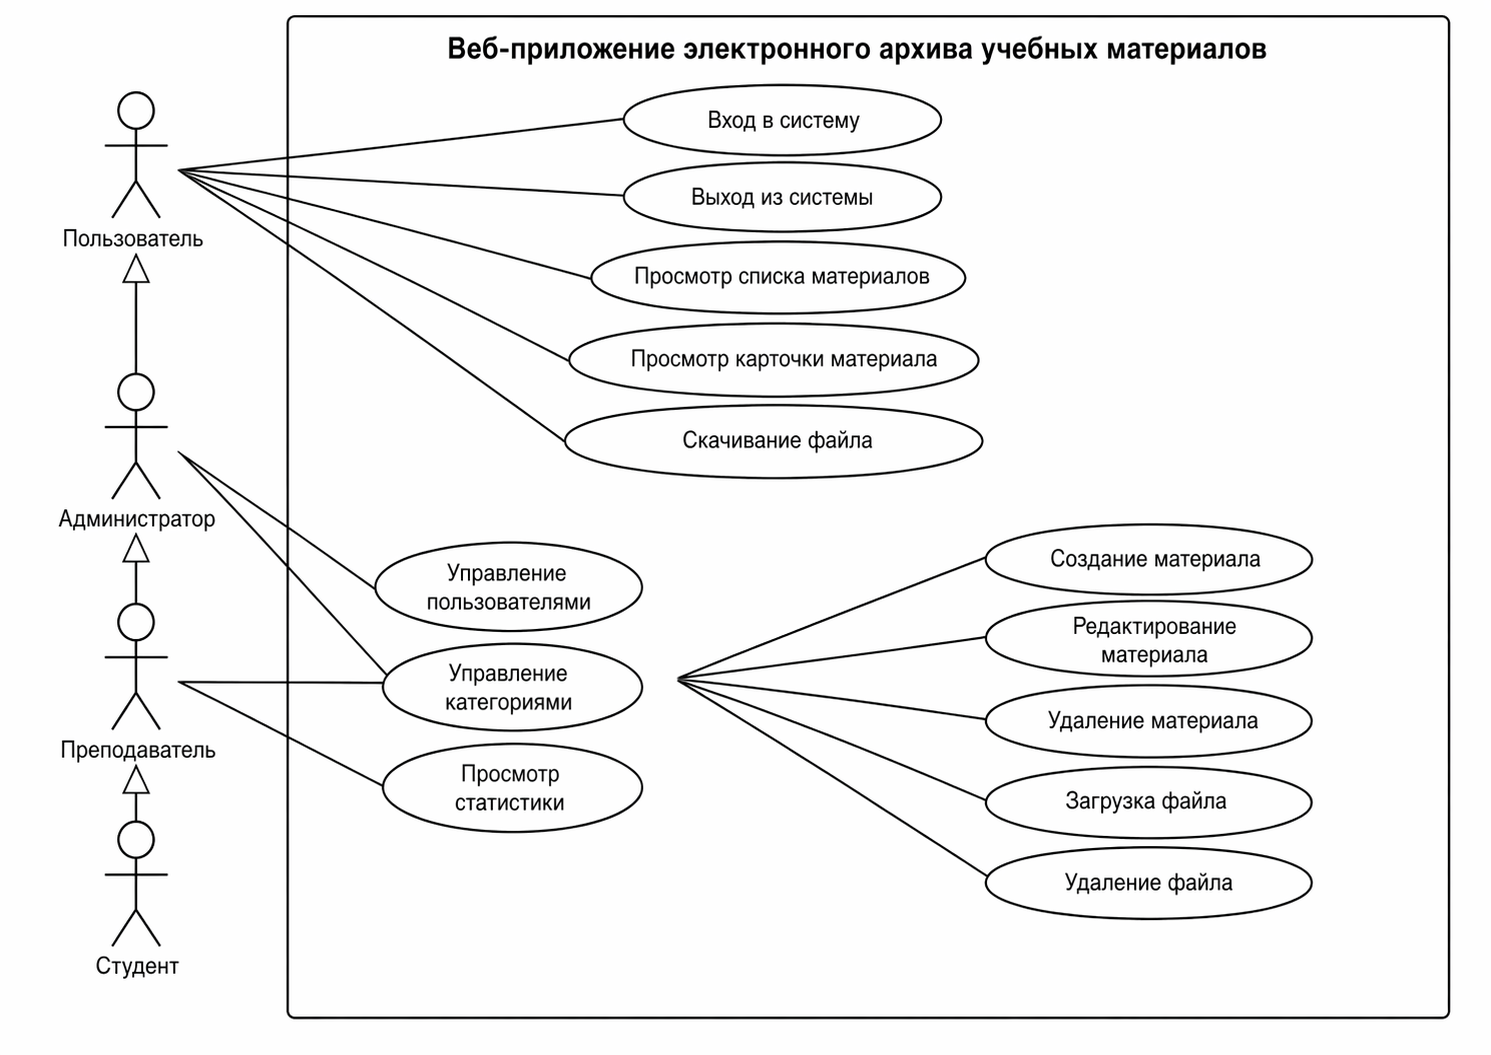
\includegraphics[width=0.92\textwidth]{images/use_case_diagram.png}
    \caption{Диаграмма вариантов использования веб-приложения}
\end{figure}

Диаграмма вариантов использования подтверждает, что проектируемая система охватывает все основные пользовательские сценарии, предусмотренные заданием: аутентификацию, разграничение прав доступа, работу с материалами и файлами, а также просмотр статистики администратором.

Для удобства навигации проектируется следующий состав страниц приложения:

\begin{longtable}{>{\raggedright\arraybackslash}p{4.2cm} >{\raggedright\arraybackslash}p{9.8cm}}
\toprule
\textbf{Страница} & \textbf{Назначение} \\
\midrule
\endfirsthead

\toprule
\textbf{Страница} & \textbf{Назначение} \\
\midrule
\endhead

\bottomrule
\endlastfoot

Главная страница & Краткая информация о системе и переход к основным разделам \\
Страница входа & Ввод логина и пароля пользователя \\
Список пользователей & Просмотр и управление учетными записями \\
Список категорий & Просмотр и администрирование категорий материалов \\
Список материалов & Просмотр всех материалов с возможностью фильтрации \\
Карточка материала & Просмотр описания материала и прикрепленных файлов \\
Страница создания и редактирования материала & Ввод названия, описания, категории и загрузка файлов \\
Страница статистики & Отображение агрегированных сведений по материалам, файлам и пользователям \\
\end{longtable}

Спроектированная функциональность приложения соответствует поставленной цели и позволяет реализовать все обязательные элементы курсового проекта.

\subsection{Проектирование модели данных для сущностей}

На этапе проектирования модели данных были выделены основные сущности предметной области: \texttt{Role}, \texttt{User}, \texttt{Category}, \texttt{Material} и \texttt{StoredFile}. Каждая из них отражает отдельный аспект работы системы.

Сущность \texttt{Role} используется для хранения названия роли и ее описания. Сущность \texttt{User} содержит данные пользователя: логин, хэш пароля, ФИО, дату создания учетной записи и ссылку на роль. Сущность \texttt{Category} предназначена для систематизации учебных материалов. Сущность \texttt{Material} хранит сведения о самом материале: название, описание, дату создания, автора и категорию. Сущность \texttt{StoredFile} содержит информацию о прикрепленных файлах: оригинальное имя, внутреннее имя хранения, путь к файлу и дату загрузки.

Связи между сущностями можно описать следующим образом:

\begin{itemize}[leftmargin=1.25cm]
    \item одной роли соответствует множество пользователей;
    \item одному пользователю может соответствовать множество материалов;
    \item одной категории может соответствовать множество материалов;
    \item одному материалу может соответствовать множество прикрепленных файлов.
\end{itemize}

Проектируемая модель данных представлена в таблице.

\begin{center}
\begin{tabularx}{0.96\textwidth}{>{\raggedright\arraybackslash}p{2.9cm} >{\raggedright\arraybackslash}p{4.8cm} >{\raggedright\arraybackslash}X}
\toprule
\textbf{Сущность} & \textbf{Основные атрибуты} & \textbf{Назначение} \\
\midrule
Role & id, name, description & Хранение ролей пользователей \\
User & id, username, password\_hash, full\_name, created\_at, role\_id & Хранение учетных записей пользователей \\
Category & id, name, description & Классификация учебных материалов \\
Material & id, title, description, created\_at, author\_id, category\_id & Описание учебного материала \\
StoredFile & id, original\_name, stored\_name, file\_path, uploaded\_at, material\_id & Хранение информации о прикрепленных файлах \\
\bottomrule
\end{tabularx}
\end{center}

Такая модель данных достаточно проста для реализации, но при этом полностью покрывает все требования.

\subsection{Проектирование структуры интерфейса и макетов основных страниц}

На этапе проектирования интерфейса была принята цель сделать приложение максимально простым и понятным. Пользователь должен быстро переходить между основными разделами системы и выполнять типовые операции без лишних действий.

В основе интерфейса лежит единый базовый шаблон страницы, содержащий верхнее меню навигации, название системы, ссылки на доступные разделы и область отображения системных сообщений. Такое решение обеспечивает единый внешний вид всех страниц приложения.

Для основных страниц были определены следующие элементы интерфейса:

\begin{itemize}[leftmargin=1.25cm]
    \item для страницы входа --- форма авторизации с полями логина и пароля;
    \item для страницы пользователей --- таблица со списком учетных записей и кнопками создания, редактирования и удаления;
    \item для страницы категорий --- таблица категорий и форма их добавления или изменения;
    \item для страницы материалов --- таблица или карточки материалов, фильтр по категории и ссылки на просмотр и редактирование;
    \item для карточки материала --- название, описание, сведения об авторе, категория, список прикрепленных файлов и кнопки действий;
    \item для страницы статистики --- набор таблиц с агрегированными данными по материалам, файлам, категориям и пользователям.
\end{itemize}

Проектируемая структура интерфейса позволяет легко масштабировать приложение и при необходимости дополнять его новыми разделами. При этом выбранный подход не перегружает пользователя и соответствует учебному характеру проекта.
\section*{Глава 3. Разработка веб-приложения}
\addcontentsline{toc}{section}{Глава 3. Разработка веб-приложения}
\stepcounter{section}

Разработанная система ориентирована на хранение, систематизацию и выдачу учебных материалов с учетом роли пользователя. В ходе разработки были реализованы базовая структура проекта, аутентификация, авторизация, механизм проверки прав доступа, CRUD-интерфейс для основных сущностей, загрузка и скачивание файлов, а также формирование статистики по материалам.

\subsection{Разработка базовой структуры приложения и шаблонов страниц}

Была сформирована базовая структура проекта, обеспечивающая разделение логики приложения, описания моделей данных, маршрутов, шаблонов страниц и конфигурации. Такой подход упрощает сопровождение программного кода и делает проект более понятным.

Структура приложения представлена следующими основными компонентами:

\begin{itemize}[leftmargin=1.25cm]
    \item файл \texttt{run.py} --- точка запуска веб-приложения;
    \item файл \texttt{config.py} --- конфигурация системы, включая путь к базе данных, папке загрузок и список допустимых расширений файлов;
    \item модуль \texttt{app/\_\_init\_\_.py} --- инициализация Flask-приложения, объекта базы данных, менеджера авторизации и вспомогательных шаблонных фильтров;
    \item модуль \texttt{app/models.py} --- описание сущностей предметной области и связей между ними;
    \item модуль \texttt{app/routes.py} --- обработка HTTP-запросов и реализация пользовательских сценариев;
    \item модуль \texttt{app/decorators.py} --- декораторы для проверки ролей пользователей;
    \item каталог \texttt{app/templates/} --- HTML-шаблоны страниц;
    \item каталог \texttt{app/uploads/} --- сохранение загруженных учебных файлов.
\end{itemize}

В файле конфигурации были заданы ключевые параметры приложения: секретный ключ, адрес базы данных SQLite, путь к каталогу загрузки файлов, максимальный размер загружаемого файла и набор разрешенных расширений. Это обеспечивает централизованное управление настройками и упрощает перенос приложения в другую среду.

Базовые шаблоны страниц построены по единому принципу: каждая страница наследуется от общего базового шаблона, содержащего навигационное меню, блок вывода сообщений системы и общую структуру пользовательского интерфейса. В результате был сформирован единый стиль страниц и обеспечено удобство навигации по разделам приложения.

В интерфейсе реализованы следующие основные страницы:

\begin{center}
\small\begin{tabularx}{0.96\textwidth}{>{\raggedright\arraybackslash}p{3.8cm} >{\raggedright\arraybackslash}X >{\raggedright\arraybackslash}p{4.3cm}}
\toprule
\textbf{Страница} & \textbf{Назначение} & \textbf{Кому доступна} \\
\midrule
Главная страница & Краткая информация о системе и последние добавленные материалы & Всем авторизованным пользователям \\
Страница входа & Ввод логина и пароля для начала работы в системе & Неавторизованным пользователям \\
Пользователи & Просмотр, создание, редактирование и удаление учетных записей & Администратору \\
Категории & Просмотр и управление категориями учебных материалов & Администратору и преподавателю \\
Материалы & Просмотр списка материалов, фильтрация и переход к карточке материала & Всем авторизованным пользователям \\
Карточка материала & Просмотр описания материала и прикрепленных файлов & Всем авторизованным пользователям \\
Статистика & Агрегированные сведения по материалам, пользователям и файлам & Администратору \\
\bottomrule
\end{tabularx}
\end{center}

Таким образом, была создана базовая структура Flask-приложения и набор шаблонов, необходимых для дальнейшей реализации предметной логики.

\subsection{Реализация аутентификации и авторизации пользователей}

Следующим этапом была реализована аутентификация пользователей. Для этого использована библиотека Flask-Login, позволяющая организовать сеансы работы пользователя, хранить состояние входа и ограничивать доступ к защищенным страницам.

В приложении реализована форма входа, содержащая поля логина и пароля. После отправки формы выполняется поиск пользователя по логину и проверка корректности пароля с использованием хэширования. В случае успешной проверки создается пользовательская сессия, после чего пользователь перенаправляется на главную страницу приложения. При ошибочном вводе данных выводится соответствующее сообщение.

Для хранения паролей используется не открытый текст, а хэш, вычисляемый средствами библиотеки Werkzeug. Это позволяет повысить безопасность приложения и соответствует типовой практике разработки веб-систем.

Ниже приведен фрагмент кода, реализующий проверку пароля в модели пользователя:

\begin{lstlisting}
def set_password(self, password: str) -> None:
    self.password_hash = generate_password_hash(password)

def check_password(self, password: str) -> bool:
    return check_password_hash(self.password_hash, password)
\end{lstlisting}

Для работы Flask-Login в проекте настроен загрузчик пользователя по идентификатору, что обеспечивает восстановление сведений о текущем пользователе из пользовательской сессии:

\begin{lstlisting}
@login_manager.user_loader
def load_user(user_id):
    return User.query.get(int(user_id))
\end{lstlisting}

После успешного входа пользователь получает доступ только к тем страницам и действиям, которые разрешены его ролью. При попытке обращения к защищенным маршрутам без авторизации система выдает сообщение о необходимости входа в систему.

Таким образом, в приложении была реализована полноценная аутентификация пользователей и базовая авторизация на уровне пользовательской сессии.

\subsection{Реализация системы проверки прав доступа в соответствии с ролью пользователя}

В разработанном приложении реализованы три роли:

\begin{itemize}[leftmargin=1.25cm]
    \item \texttt{admin} --- администратор;
    \item \texttt{teacher} --- преподаватель;
    \item \texttt{student} --- студент.
\end{itemize}

Роль пользователя хранится в отдельной сущности \texttt{Role}, а в сущности \texttt{User} предусмотрена связь с соответствующей записью роли. Для проверки ролей в модели пользователя реализован метод \texttt{has\_role()}, возвращающий истинное значение, если роль пользователя входит в заданный набор.

Для ограничения доступа к маршрутам был создан собственный декоратор \texttt{roles\_required}. Он используется совместно с декоратором \texttt{@login\_required} и проверяет, обладает ли текущий пользователь допустимой ролью. Если пользователь не авторизован, возвращается код 401, а если его роль не соответствует требуемой, возвращается код 403.

\begin{lstlisting}
def roles_required(*role_names):
    def decorator(view_func):
        @wraps(view_func)
        def wrapped(*args, **kwargs):
            if not current_user.is_authenticated:
                abort(401)
            if not current_user.has_role(*role_names):
                abort(403)
            return view_func(*args, **kwargs)
        return wrapped
    return decorator
\end{lstlisting}

Кроме проверки роли на уровне маршрута, для операций над материалами реализована дополнительная проверка принадлежности материала пользователю. Это необходимо для того, чтобы преподаватель мог редактировать и удалять только собственные материалы, тогда как администратор может управлять всеми материалами.

Следовательно, в приложении реализовано ролевое разграничение доступа, полностью соответствующее требованиям.

\subsection{Реализация CRUD-интерфейса для пользователей, категорий и материалов}

В приложении реализованы операции создания, просмотра, редактирования и удаления для трех основных сущностей: пользователей, категорий и материалов. Все операции доступны через веб-интерфейс и соответствующие маршруты Flask.

\subsubsection*{CRUD для пользователей}

Управление пользователями доступно только администратору. Он может просматривать список учетных записей, создавать новых пользователей, изменять логин, ФИО, пароль и роль, а также удалять пользователей. Для защиты системы предусмотрено ограничение, запрещающее администратору удалить собственную учетную запись во время работы в системе.

\subsubsection*{CRUD для категорий}

Категории используются для систематизации учебных материалов. Администратор может создавать новые категории, изменять их название и описание, а также удалять категории. При этом реализована проверка, запрещающая удаление категории, если с ней уже связаны материалы. Такое ограничение поддерживает целостность данных.

\subsubsection*{CRUD для материалов}

Материал является основной сущностью приложения. При создании материала указываются его название, описание и категория. Автором материала автоматически становится текущий авторизованный пользователь. После создания материал отображается в общем списке и доступен для просмотра пользователям с соответствующими правами.

При редактировании материала допускается изменение названия, описания и категории, а также добавление новых файлов. В режиме редактирования отображается список уже загруженных файлов, для которых реализованы отдельные действия по скачиванию и удалению.

Основные CRUD-маршруты приложения представлены в таблице.

\begin{center}
\footnotesize\begin{tabularx}{0.96\textwidth}{>{\raggedright\arraybackslash}p{6.0cm} >{\raggedright\arraybackslash}X >{\raggedright\arraybackslash}p{1.6cm}}
\toprule
\textbf{Маршрут} & \textbf{Назначение} & \textbf{Методы} \\
\midrule
/users & Список пользователей & GET \\
/users/create & Создание пользователя & GET, POST \\
/users/{id}/edit & Редактирование пользователя & GET, POST \\
/users/{id}/delete & Удаление пользователя & POST \\
/categories & Список категорий & GET \\
/categories/create & Создание категории & GET, POST \\
/categories/{id}/edit & Редактирование категории & GET, POST \\
/categories/{id}/delete & Удаление категории & POST \\
/materials & Список материалов и фильтрация & GET \\
/materials/create & Создание материала & GET, POST \\
/materials/{id} & Карточка материала & GET \\
/materials/{id}/edit & Редактирование материала & GET, POST \\
/materials/{id}/delete & Удаление материала & POST \\
\bottomrule
\end{tabularx}
\end{center}

Таким образом, в системе реализован полноценный CRUD-интерфейс для основных сущностей предметной области.

\subsection{Реализация загрузки, скачивания и удаления файлов учебных материалов}

Одной из ключевых функций приложения является работа с учебными файлами. Для этого в проекте реализована отдельная сущность \texttt{StoredFile}, содержащая оригинальное имя файла, внутреннее имя для хранения, путь к файлу на диске, дату загрузки и связь с материалом.

При загрузке файла выполняется проверка расширения. Разрешены только типы файлов, соответствующие учебным материалам: PDF, DOC, DOCX, TXT, PPT, PPTX, XLS, XLSX, PNG, JPG, JPEG. После проверки файл сохраняется в каталог \texttt{app/uploads}. Для предотвращения конфликтов имен и перезаписи существующих файлов используется генерация уникального имени на основе UUID.

Фрагмент кода сохранения файлов имеет следующий вид:

\begin{lstlisting}
original_name = secure_filename(file.filename)
extension = original_name.rsplit('.', 1)[1].lower()
stored_name = f"{uuid.uuid4().hex}.{extension}"
file_path = os.path.join(upload_folder, stored_name)
file.save(file_path)
\end{lstlisting}

Скачивание файла реализовано отдельным маршрутом. При обращении к нему сервер находит файл по идентификатору и отправляет его пользователю как вложение, сохраняя исходное имя файла для скачивания.

Удаление файла также выполняется отдельным маршрутом. При этом сначала удаляется физический файл с диска, затем удаляется соответствующая запись из базы данных. Возможность удаления предоставляется только администратору или преподавателю, имеющему право управления данным материалом.

Реализованный механизм загрузки, скачивания и удаления файлов позволяет полностью закрыть одно из обязательных требований, связанное с обработкой файловых данных.

\subsection{Реализация агрегирования данных и формирования статистики по материалам}

Для выполнения требования, связанного с обработкой и агрегированием данных, в приложении была реализована отдельная страница статистики. Доступ к ней предоставляется только администратору.

На странице статистики формируются следующие агрегированные показатели:

\begin{itemize}[leftmargin=1.25cm]
    \item общее количество материалов в системе;
    \item общее количество загруженных файлов;
    \item количество материалов по категориям;
    \item количество материалов по авторам;
    \item количество пользователей по ролям.
\end{itemize}

Для формирования статистики используются агрегатные функции SQLAlchemy, в частности \texttt{COUNT()}, а также операции группировки по категориям, авторам и ролям. Пример формирования статистики по категориям представлен ниже:

\begin{lstlisting}
materials_by_category = (
    db.session.query(Category.name, func.count(Material.id))
    .outerjoin(Material, Material.category_id == Category.id)
    .group_by(Category.id)
    .order_by(Category.name)
    .all()
)
\end{lstlisting}

Полученные значения передаются в шаблон страницы статистики и выводятся в виде наглядных таблиц. Это позволяет администратору оценивать наполнение архива, распределение материалов по категориям и активность пользователей.

\subsection{Тестирование основных пользовательских сценариев и проверка прав доступа}

После завершения реализации основных модулей приложения было выполнено функциональное тестирование пользовательских сценариев. Целью тестирования являлась проверка корректности работы разработанного веб-приложения в условиях, приближенных к его реальному использованию, а также подтверждение выполнения требований курсового проекта, связанных с аутентификацией, авторизацией, разграничением прав доступа, CRUD-операциями, обработкой файлов и формированием статистики.

Тестирование проводилось методом последовательной ручной проверки ключевых пользовательских сценариев. В качестве тестовых ролей использовались три учетные записи: администратор, преподаватель и студент. Проверка включала как позитивные сценарии, при которых пользователь выполняет допустимые действия, так и негативные сценарии, при которых система должна запретить доступ к функции или странице. Основное внимание уделялось корректности маршрутизации, сохранению данных в базе, изменению интерфейса в зависимости от роли пользователя, а также работе операций загрузки, скачивания и удаления файлов.

Для проверки были подготовлены тестовые данные: несколько пользователей с различными ролями, набор категорий учебных материалов, несколько записей материалов и прикрепленные к ним файлы разных типов. После каждого действия проверялось не только визуальное изменение данных на странице, но и фактическое наличие или отсутствие соответствующих записей в базе данных и файловом хранилище приложения.

Результаты тестирования основных сценариев приведены ниже.

\begin{longtable}{>{\centering\arraybackslash}p{0.9cm} >{\raggedright\arraybackslash}p{5.5cm} >{\raggedright\arraybackslash}p{4.2cm} >{\raggedright\arraybackslash}p{4.0cm}}
\toprule
\textbf{№} & \textbf{Проверяемый сценарий} & \textbf{Ожидаемый результат} & \textbf{Фактический результат} \\
\midrule
\endfirsthead
\toprule
\textbf{№} & \textbf{Проверяемый сценарий} & \textbf{Ожидаемый результат} & \textbf{Фактический результат} \\
\midrule
\endhead
1 & Открытие защищенной страницы без авторизации & Система перенаправляет пользователя на страницу входа & Выполнено, доступ без входа не предоставляется \\
2 & Вход администратора по корректным учетным данным & Открывается главная страница приложения, пользовательская сессия создается & Выполнено, вход успешен \\
3 & Выход из системы & Сессия пользователя завершается, защищенные страницы снова недоступны & Выполнено, повторный доступ требует авторизации \\
4 & Создание нового пользователя администратором & В базе появляется новая учетная запись с выбранной ролью & Выполнено, пользователь создается и отображается в списке \\
5 & Редактирование данных пользователя администратором & Измененные значения сохраняются и отображаются в интерфейсе & Выполнено, обновленные данные отображаются корректно \\
6 & Удаление пользователя администратором & Учетная запись удаляется из базы и исчезает из списка & Выполнено, запись удаляется корректно \\
7 & Создание категории администратором & Новая категория сохраняется и доступна при создании материалов & Выполнено, категория появляется в списке \\
8 & Попытка студента открыть страницу категорий & Доступ запрещается, страница недоступна студенту & Выполнено, доступ студенту ограничен \\
9 & Создание нового материала преподавателем & Материал сохраняется с указанием автора и категории & Выполнено, материал добавляется в систему \\
10 & Редактирование материала его автором & Изменения сохраняются и отображаются на странице просмотра материала & Выполнено, материал обновляется корректно \\
11 & Попытка студента изменить существующий материал & Система запрещает выполнение операции & Выполнено, права студента ограничены \\
12 & Загрузка файла при создании или редактировании материала & Файл сохраняется на сервере и отображается в карточке материала & Выполнено, файл доступен в списке вложений \\
13 & Скачивание прикрепленного файла авторизованным пользователем & Браузер начинает загрузку выбранного файла & Выполнено, файл скачивается корректно \\
14 & Удаление файла из карточки материала пользователем с соответствующими правами & Файл удаляется из хранилища и перестает отображаться в интерфейсе & Выполнено, удаление работает корректно \\
15 & Открытие страницы статистики администратором & Отображаются агрегированные показатели по материалам, файлам и пользователям & Выполнено, статистика формируется корректно \\
16 & Попытка преподавателя открыть страницу статистики & Доступ запрещается, страница статистики недоступна преподавателю & Выполнено, доступ ограничен \\
17 & Попытка студента открыть страницу статистики & Доступ запрещается, страница статистики недоступна студенту & Выполнено, доступ ограничен \\
18 & Проверка отображения автора материала в интерфейсе & Для каждого пользователя отображается формат ``ФИО (логин)'' & Выполнено, отображение авторов единообразно \\
19 & Проверка отображения времени создания записей & Дата и время выводятся с учетом часового пояса МСК (UTC+3) & Выполнено, время отображается корректно \\
20 & Проверка агрегированных данных после добавления новых материалов и файлов & Количественные показатели изменяются в соответствии с новыми данными & Выполнено, статистика обновляется корректно \\
\bottomrule
\end{longtable}

По результатам проведенного тестирования можно сделать вывод, что основные пользовательские сценарии выполняются корректно. Проверка показала, что приложение устойчиво отрабатывает как обычные операции пользователя, так и ограничения, связанные с ролью учетной записи. Особенно важным результатом является подтверждение того, что студент не имеет доступа к административным функциям, преподаватель не может просматривать статистику, а изменение и удаление материалов и файлов доступно только пользователям, обладающим соответствующими правами.

Также в процессе тестирования были выявлены и устранены отдельные недочеты интерфейса и серверной логики. К ним относились вопросы отображения времени, единообразного показа имени пользователя в формате ``ФИО (логин)'', а также корректная обработка удаления уже загруженных файлов со страницы редактирования материала. После внесения исправлений указанные сценарии были протестированы повторно и подтвердили корректность реализации.

% Заключение
\section*{Заключение}
\addcontentsline{toc}{section}{Заключение}

В результате выполнения курсового проекта было разработано веб-приложение для хранения, систематизации и публикации учебных материалов с ролевым разграничением доступа. В ходе работы была проанализирована предметная область, рассмотрены существующие подходы к организации электронных архивов учебных материалов, а также выбран технологический стек, включающий Python, Flask, Flask-Login, Flask-SQLAlchemy, SQLite, Jinja2 и Bootstrap.

На этапе проектирования были определены роли пользователей, основные сценарии использования системы, структура интерфейса и модель данных для сущностей, связанных с хранением материалов и файлов. На этапе разработки была реализована базовая структура приложения, аутентификация и авторизация пользователей, проверка прав доступа в соответствии с ролью, CRUD-интерфейс для пользователей, категорий и материалов, механизм загрузки, скачивания и удаления файлов, а также страница статистики с агрегированными данными.

Проведенное тестирование основных пользовательских сценариев подтвердило корректность работы реализованного приложения. Система обеспечивает доступ к функциям в соответствии с ролью пользователя, поддерживает работу с материалами и файлами и удовлетворяет обязательным требованиям курсового проекта. Полученный результат может рассматриваться как работоспособная основа для дальнейшего расширения системы, например для добавления более сложного поиска, журналирования действий пользователей, расширенной аналитики и интеграции с иными образовательными сервисами.

% Список литературы
\renewcommand{\refname}{Список использованных источников}
\phantomsection
\addcontentsline{toc}{section}{Список использованных источников}
\nocite{*}
\bibliographystyle{ugost2008}
\bibliography{refs}

% Приложение
\startappendix

\section*{Приложение А}
\addcontentsline{toc}{section}{Приложение А}
\stepcounter{section}

В приложении приведена диаграмма вариантов использования разработанного веб-приложения, отражающая основные роли пользователей и ключевые сценарии взаимодействия с системой.

\begin{figure}[ht!]
    \centering
    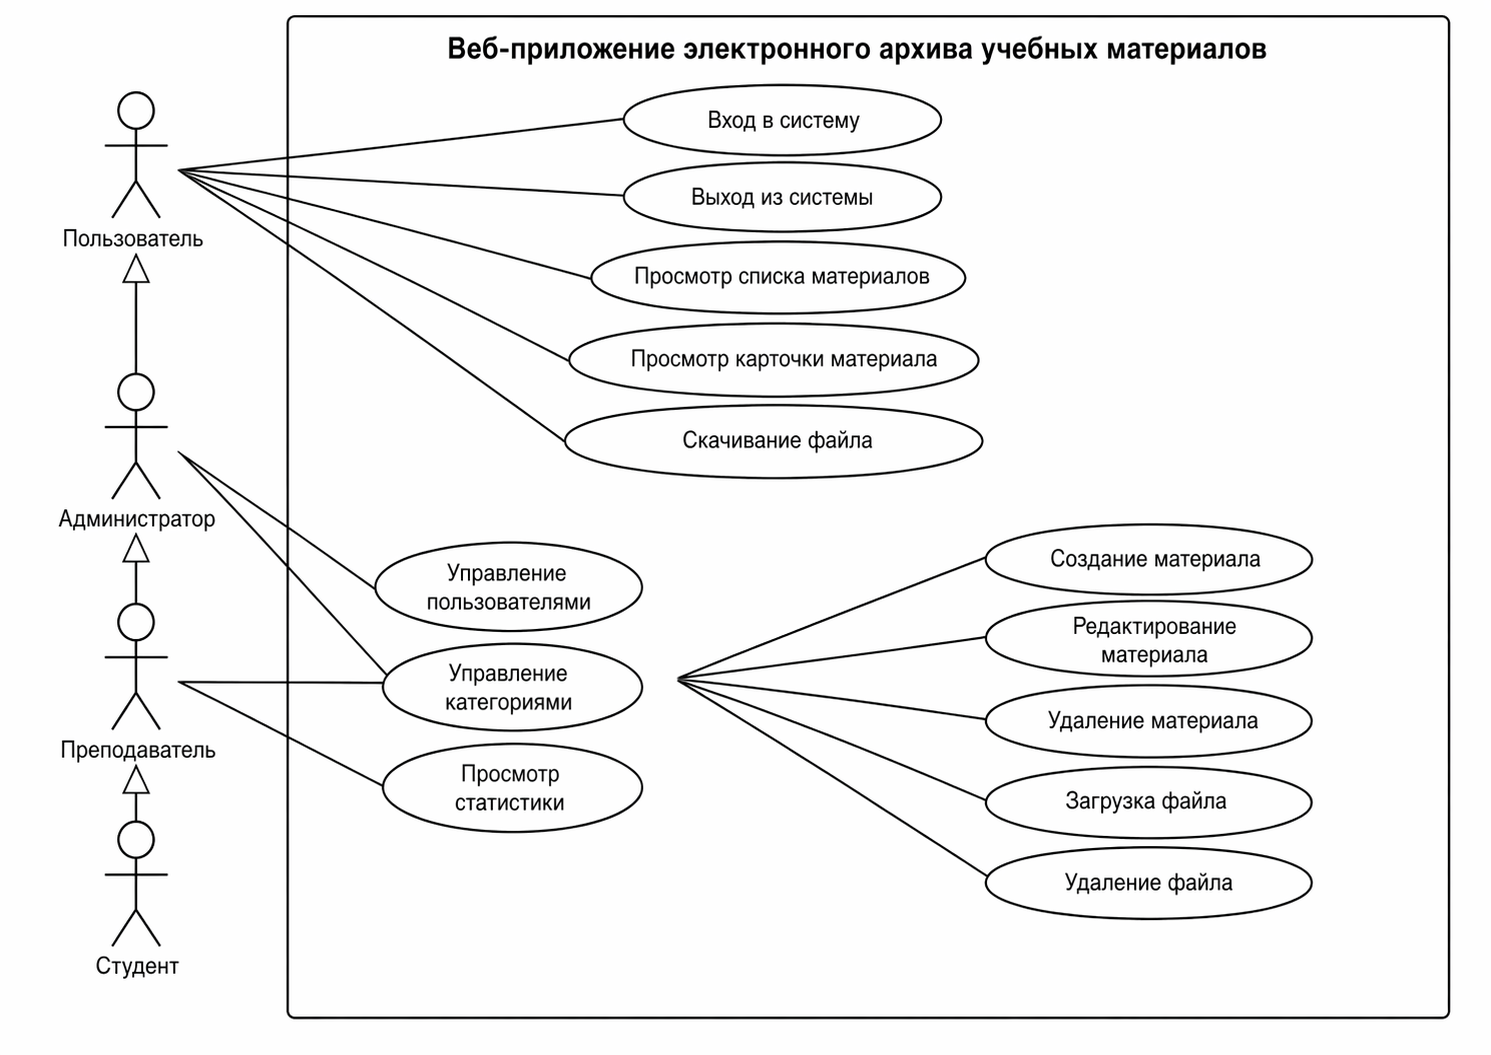
\includegraphics[width=0.95\textwidth]{images/use_case_diagram.png}
    \caption{Диаграмма вариантов использования веб-приложения}
\end{figure}

\end{document}